% 
% Annual Cognitive Science Conference Format


\documentclass[10pt,letterpaper]{article}

\usepackage{mathtools}
\usepackage{cogsci}
\usepackage{pslatex}
\usepackage{apacite}


\title{A Bayesian Framework for Learning Regular Expressions}
 
\author{{\large \bf{P. Thomas Barthelemy} (bartho@stanford.edu)} \\
  Department of Computer Science, 353 Serra Mall \\
  Stanford, CA 94305 USA
  \AND {\large \bf Nicholas Borg (nickborg@stanford.edu)} \\
  Symbolic Systems Program, Margaret Jacks Hall \\
  Stanford, CA 94305 USA}


\begin{document}

\maketitle


\begin{abstract}
Regular expressions are used to define a set of strings that match a certain pattern. In the following experiment, we posit that the means by which humans judge similarity of words can be represented by a method of inference using regular expressions. In short, there is a tradeoff of generality and specificity that allows for a selection of an optimal regular expression to categorize a list of input strings.

\textbf{Keywords:} 
Model inference, regular expression.
\end{abstract}


\section{Overview and Motivation}
Understanding the human ability to find structure in data is integral to both cognitive psychology and artificial intelligence. In recent years, a number of studies have shown that human inference across a number of tasks may be Bayesian at some level of analysis. 
Inspired by Tennenbaum's treatment of the number game, we propose a regular expression game as follows: Given a set $S$ of input strings drawn from a language $L$, what is the likelihood that a new string $s$ is in $L$. Playing such a game requires inferring the rules that govern $L$ from $S$. Noting that humans perform this task  with success on a daily basis in writing regular expressions to process string data, we considered the hypothesis that human inference of regular expressions is at some level Bayesian. 

In doing so, we first generated a Bayesian model that, given a set of input strings $S$, generated a regular expression that describes $S$ with the highest posterior probability. This model is discussed in the first part of this paper. We then ran a behavioral experiment in which subjects were asked whether or not a given string $s$ fits with a set of strings $S$. We compare the result of that experiment with results generated given an extension of our model.  

\section{Description of the Model}

%\subsection{Balancing Generality with Specificity}
Our model has two parts: We generate a set of regular expressions which describe a set of input stings $S$, and we find the regular expression in that set with the highest posterior probability. The posterior probability is proportional to the product of the hypothesis' prior probability and its likelihood.
\begin{align*}
	p(h|S) \propto p(h) p(S|h)
\end{align*}
Below, we define the prior probability such that our model biases smaller hypotheses, and the likelihood of generating a given hypothesis is inversely proportional to its cost. Our model aims to balance generality with specificity. For example, given "ABC, ABD", we wish to favor the regex $AB(C|D)$ over "?*", which is less likely given the size principle. At the same time, given "ABA", "ABC", "ABD", "ABE", "ABF", we may wish to favor 'AB?' over  '$AB(A|C|D|E|F)$'

\subsection{Representation of Hypotheses}
Regular expressions are equivalent to deterministic finite automata (DFA).\footnote{See the Appendix for a brief summary of our regex notation.} Because DFA are often easier to reason with, we use them to represent regular expressions in our model (See Fig 1 for an example DFA.)

Further, we define the probability with which a DFA would stop generating a string at a start state . For instance, given the regular expression \verb!a*!, we would need to define the probability of generating strings \verb!a!, \verb!aa!, \verb!aaa!, etc.

In this sense, our DFA is similar to a probabilistic automaton, although the acceptance criteria is $\tau=0$, so the languages represented by our DFA are still regular. [Citation]. A second difference is that there is no concept of stopping string generation in probabilistic automaton.

% TODO: explain character scope!

\subsection{Generating Hypotheses}
The hypothesis space is initiated with the base hypothesis, the term applied to a DFA that accepts strictly the input strings. Next, hypotheses are added to the hypothesis space through two processes of generalization: merging and applying wildcards.

\subsubsection{Merging} Merging is the process of combining states of a DFA. The newly create state has all incoming and outgoing transitions of its predecessors. Thus, the DFA will continue to accept the same set of strings as the original DFA. However, the DFA will often accept more strings after merging, thus merging states results in a more generalized DFA.

If merging is continued, the DFA will eventually have only one state with all transitions leading to itself. Such a state accepts all strings containing only zero or more of the original characters. A series of merges are illustrated in Figure~\ref{merge-figure}.

\begin{figure}[ht]
\begin{center}
\begin{align*}
\text{(a)}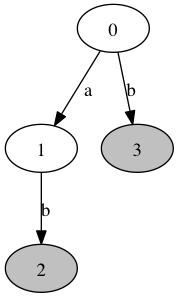
\includegraphics[scale=0.4]{merge-0.png}
&\text{(b)}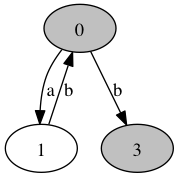
\includegraphics[scale=0.4]{merge-1.png}
&\text{(c)}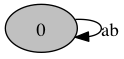
\includegraphics[scale=0.4]{merge-2.png}
\end{align*}
\end{center}
\caption{An example of state merging. The DFA starts at state 0 and accepts only at the shaded states. The base hypothesis accepts ``b'' and ``ab'' (a). After merging states 0 and 2, the next DFA accepts an infinite set of strings (b). Finally, the merge of states 0 and 1 forces the merge of state 0 and 3 to maintain one unique outbound transition for any state and character (c).} 
\label{merge-figure}
\end{figure}

% TODO: mention anti-unification

\subsubsection{Wildcards} Wildcards generalize the DFA by extending state transitions to apply to a class of characters. Figure~\ref{wildcard-figure} illustrates an example of this.

\begin{figure}[ht]
\begin{center}
\begin{align*}
\text{(a)}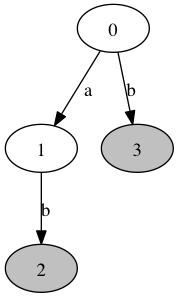
\includegraphics[scale=0.4]{wildcard-0.png}
&\text{(b)}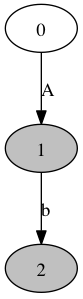
\includegraphics[scale=0.4]{wildcard-1.png}
\end{align*}
\end{center}
\caption{An example of inserting a wildcard, ``A'', which represents any character. Replacing a wildcard for one of the outbound transitions of state 0 has forced a merge of states 1 and 3.} 
\label{wildcard-figure}
\end{figure}

\subsubsection{Enforcing Determinism} Merging states and replacing transitions with wildcards can allow one state to have non-unique outbound transitions. However, this turns our representation into a nondeterministic finite automaton (NFA) instead of a DFA. Both are equivalent, but the latter afford easier manipulation for our experiment. Thus, to convert the NFA back to a DFA, we use the subset construction, the effect of which is illustrated in both Figure~\ref{merge-figure} and Figure~\ref{wildcard-figure}.

\subsection{Searching the Hypothesis Space} The number of hypotheses grows quickly with the number of states in the base hypothesis. As a lower bound, the number of hypotheses is at least as large as the number of possible starting nodes. Because the starting node could be merged with any subset of the remaining $n-1$ nodes in the DFA, there are $2^{n-1}=\Omega(2^n)$ possible start states. Thus, the hypothesis space is at least exponential in the number of starting nodes in the regular expression.

Similarly, the number of possible regex variants created by simply replacing transitions with wildcards is given by $2^m$ where $m$ is the number of transitions. Thus, simply modifying expressions to include wildcards is also exponential.

An upper bound for the complexity of model merging is much more extreme. Performing subset construction for an NFA with $n$ states can produce, in the worst case, a DFA with $2^n$ states. Assuming that any subset of these states also produces a valid DFA, we can have at most $2^{2^n-1}$ DFA.
% \footnote{See the Appendix for detailed sizing of the hypothesis space.} Actually, this seems inaccurate.

We resolve this issue by performing beam search. In beam first, we perform breadth first search, but for any given depth of the search tree, we only consider children of the $m$ most promising hypotheses. In our case, the most promising hypotheses were defined as those with the highest posterior probability. 

\section{Inference with DFA}
The posterior probability for a DFA as a hypothesis is given by the following.
\begin{align*}
	p(h|S) \propto p(S|h)p(h)
\end{align*}
Thus, inferring the best DFA given a set of input strings was essentially a problem in balancing simplicity with conservation of belief. That is, DFA were biased a priori for being simpler, but simpler DFA tended to accept more strings.

\subsection{Prior Probability}
We assigned the prior probability to the hypotheses (i.e. regexes) based on the size of the DFA and the number of transitions. In the following equation, $|S|$ is the number of states in the DFA and $|T|$ is the number of tranisitons in the DFA, where a wildcard counts as only one transition. 
\begin{align*}
	P(h) \propto e^{-\alpha|S| - \beta|T|}
\end{align*}
Thus, we have biased smaller DFA that use wildcards instead of literal characters. [cite Program Merging model]

\subsection{Likelihood}
To define the likelihood of producing certain strings, we turn a DFA into a generative automaton that has a probability of generating a given string. Letting the input strings be independent, the probability of generating strings $S$ is equal to the product of the probabilities of generating each string.
\begin{align*}
	p(S) = \prod_{s \in S} p(s)
\end{align*}

Let the $s$ be the concatenation of characters $a_1a_2...a_n$. We define the probability of generating a string as the product of the probability of generating the letters in sequence $p(a_1a_2...a_n)$ and the product of stopping the string generation on an accept state $p(\text{stop})$.
\begin{align*}
	p(s) = p(a_1a_2...a_n)p(\text{stop})
\end{align*}

We define the probability of generating the characters as the product of the probabilities of making each state transition over each state.
\begin{align*}
	p(a_1a_2 ... a_n) = \prod_{i=1}^{n}p(\delta(r_i, a_{i+1}))
\end{align*}
where $r_i$ is the state reached after the first $i-1$ characters, and $r_1$ is the start state.

To simplify inference, we assume uniform probability over all possible state transitions. Formally, the probability of making a state transition is given by:
\begin{align*}
	p(\delta(r_i, a_{i+1})) &= \frac{1}{\sum_{a\in A} 1\{\delta(r_i, a)\}}
\end{align*}
Notice that the denominator counts the number of characters for which a transition is defined. In the case of a wildcard, the transition is defined for all 26 letters.

For the cases in which a string may alternatively be accepted or continue, one must assign a probability for accepting or continuing the string. For instance, consider the DFA in part (c) of Figure~\ref{merge-figure}. The DFA may generate the empty string, \verb!E!, or it may generate any arbitrary string with \verb!a! and \verb!b!, like \verb!ababbba!. We define the probability of stopping at a given string to be a fixed value $\tau$. This makes shorter strings more likely to be generated.

Instead of leaving $\tau$ as a parameter of the model, we assume a uniform prior over the parameter and marginalize it when calculating the likelihood of a string. So, let $b$ be the number of times the DFA skipped an accept state before accepting. That is, $b$ is given by the equation below, where $F$ is the set of accept states.
\begin{align*}
	b = \sum_{i=1}^{n-1} 1 \{ r_i \in F\}
\end{align*}

% TODO: Cite this

The probability of stopping at an accept state is given by the equation below. The condition $\exists a : \delta(r_n, a)$ indicates that there is an outbound transition for the accept state of the string.
\begin{align*}
	p(\text{stop}) &= \left\{
		\begin{array}{rl}
		\tau (1-\tau)^b & r_n \in F \wedge \exists a : \delta(r_n, a)
		\\ (1-\tau)^b & r_n \in F \wedge \not \exists a : \delta(r_n, a)
		\\ 0 & \text{otherwise}
		\end{array}
		\right.
\end{align*}

Marginalizing over all possible values of $\tau$, we have:
\begin{align*}
	\int_0^1 \tau (1-\tau)^b &= \frac{1}{b^2+3b+1}
	\\ \int_0^1 (1-\tau)^b &= \frac{1}{b+1}
\end{align*}

Our equation for $p(\text{stop})$ is thus:
\begin{align*}
	p(\text{stop}) &= \left\{
		\begin{array}{rl}
		\frac{1}{b^2+3b+1} & \in F \wedge \exists a : \delta(r_n, a)
		\\ \frac{1}{b+1} & \in F \wedge \not \exists a : \delta(r_n, a)
		\\ 0 & \text{otherwise}
		\end{array}
		\right.
\end{align*}

\section{Experiment Design and Model Fitting}
Having generated the above Bayesian model for selection of the regular expression with the highest posterior probability, we then conducted a behavioral experiment.  41 subjects (Median age 34, std-dev 13.3) were surveyed on Amazon Mechanical Turk. Two groups (one of twenty, one of 21) were presented with 10 yes or no questions in which they were asked to determine whether a given string `fit' with a list of strings. A sample question was as follows: \\
\begin{center}Given the list:

\textbf{yyyt \\
yt \\
yyyt \\
yyyt \\ 
yt}

Does \textbf{yyt} fit?
\end{center}

The experimental data served two purposes. Using the responses to four out of 23 questions, we set the parameters for alpha and beta. We then used the remaining questions to test our model's performance in a regex game as shown below. 

\subsection{Parameter Fitting}
Because the role of $\beta$ had the effect of biasing models with fewer transitions, it also had a tendency to bias regular expressions with fewer states. For instance, the $\beta$ term would prefer the regular expression \verb!a*! over \verb!aaaa!. Thus, this term was fitted before fitting the $\alpha$ term.

To fit the $\beta$ term, we observed experiments that would indicate the transition point between a preference for generality over specificity for wildcard-based experiments (e.g. the first two experiments outlined in Table~\ref{parameter-table}). Utilizing the fact that increasing the ratio of repeated strings to new strings decreases the likelihood of a wildcard, and decreasing the length of the sample strings would increases the likelihood of a wildcard, the first two experiments suggest a decision point. That is, if the DFA model is a valid representation of the subjects' responses, then the $\beta$ term should be between $3$ and $5$. For further experimentation, we fixed it at $4$.

Fitting the $\alpha$ term was less clear. In particular, the desired behavior was easily observed with $\alpha=0,\beta=4$. However, a term of $\alpha=1$ was used to bias hypotheses with fewer states given the same number of transitions.

% TODO: move this?
\begin{table}[!ht]
\begin{center} 
\caption{Parameter fitting experiments} 
\label{parameter-table} 
\vskip 0.12in
\begin{tabular}{llll} 
\hline
Input  & Test & Subject Accept & Model Accept
% \\ \hline
% bhi, bhw, bhi, & bho & 30\% & $\beta < 14$
% \\ bhw, bhw
\\ \hline
efg, hfg, ifg & ffg & 45\% & $\beta > 3$
\\ \hline
glts, elts, glts, & ilts & 70\% & $\beta > 5$
\\ flts
\\ \hline
ab, abb & abbb & 90\% & $\alpha = 0, \beta = 4$
\\ \hline
ao, aoo, aooo & aoooo & 80\% & $\alpha = 0, \beta=4$
\\ \hline
\end{tabular} 
\end{center} 
\end{table}

\subsection{The Regex Game}
Given the fitted model, we then considered the following task: 

Given a language $\mathcal{L}$, a set of regular expressions $\mathcal{H}$ (where these are candidates for $\mathcal{L}$), a set of strings drawn $S$ from $\mathcal{L}$, and a string $s$, we define

\begin{align*}
	p(s \in \mathcal{L} | S \subseteq {L}) = \sum_{h \in \mathcal{H}} 1 (s \in h) p(h|S)
\end{align*}

For human participants, because the hypothesis is unobserved, we take $p(s \in \mathcal{L} | S \subseteq {L}) $ to be the average acceptance of a test string given a set $S$. 

In our model, we consider $\mathcal{H}$ to be the set of all hypotheses generated in our model.

\section{Results and Discussion}
Figure 3 shows the comparison between our model and the human subject data.

\begin{figure}[ht]
\begin{center}
\begin{align*}
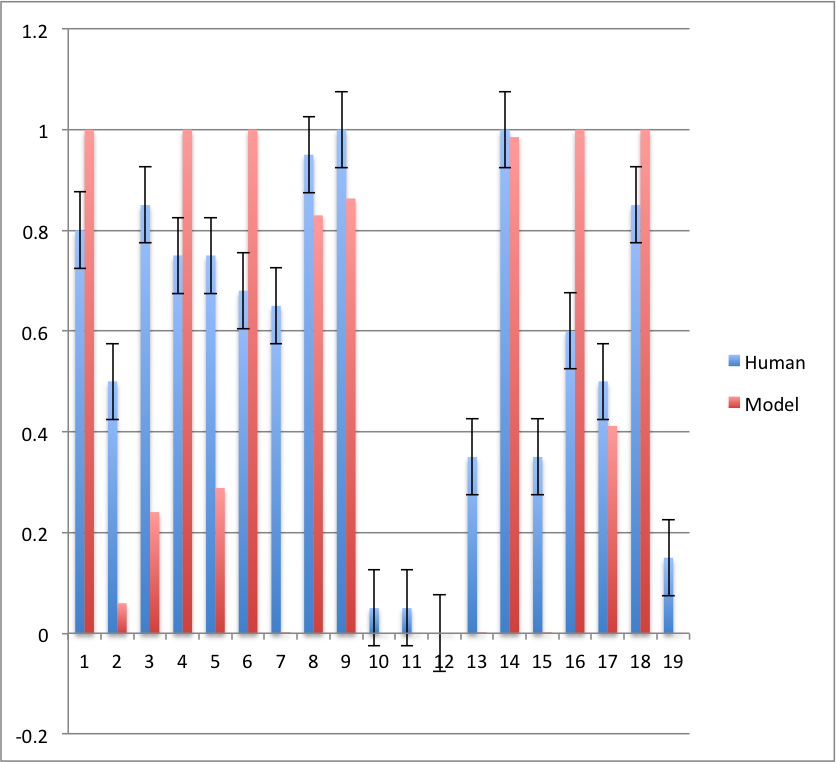
\includegraphics[scale=0.6]{results.png}
\end{align*}
\end{center}
\caption{Chart showing  $p(s \in \mathcal{L} | S \subseteq {L}) $. Human subject data is in red, model data is in blue. $R$ = .75} 
\label{merge-figure}
\end{figure} 

We note that subjects completed the 10 or 11 question survey on average in around three minutes. It remains unclear if more standardized results would have emerged in certain cases if subjects had taken more time with the task. In addition, more fine grained results may have been obtained if we had instead allowed users to bet certain amounts on whether or not a test string was in $S$. 


We note that in cases 1 (S = \{'yyyt', 'yt', 'yyyt', 'yyyt', 'yt'\}, s= 'yyyyyt' ), 4( S = \{jojojojo', 'jojojojo', 'jojojojo'\}, s = jojo), and 6 (s =  tw,  S = \{'twtwtw', 'twtwtw', 'twtwtw'\}), it is clear that the model weighs a smaller number of transitions greater than human subjects do. However, because this same parameter in part controls for wildcards, lowering it reduces performance on many other cases. This suggests that our model's parameter $\beta$ may in fact be better represented by more than one variable in human decision making. 

We also observe that in such cases, there was a relatively small set of probable hypotheses, and that any favoring of smaller hypotheses was magnified by this fact. 
\section{Conclusion and Future Work}

Despite the number of ways in which our model might be improved mentioned above,  it remains highly implausible that the brain generates its set of candidate hypotheses by ever considering even $2^n$ hypotheses in the first level of beam search we perform, much less far more than that. Doing so would be highly inefficient: the number of implausible hypotheses generated would in most cases be far greater than the number of `good' hypotheses. Far more plausible a priori is the hypothesis that the brain uses of number of heuristics to generate a certain set of candidate hypothesis, and then uses some process analogous to Bayesian inference to select among those hypotheses. To shed light on how this hypothesis selection process may occur, we designed an experiment in which candidates chose among a number of possible rules to explain a set of strings S, but have yet to gather enough data to reach any significant conclusions. 

Further experiments could be conducted to determine what heuristics may be at work in the hypothesis generation process. For any set of candidate heuristics, it will remain to be determined whether or not such heuristics are at some point learned. Clearly some are when semantic considerations are at work: cat and mat but not qat are meaningful english words; 'ao' and 'eo' and 'io' begin with vowels unlike 'xo'. This experiment was designed to avoid such candidate hypotheses. 




% \section{General Formatting Instructions}

% For standard spoken papers and standard posters, the entire contribution (including figures, references, everything) can be no longer than six pages. For abstract posters, the entire contribution can be no longer than one page. For symposia, the entire contribution can be no longer than two pages.

% The text of the paper should be formatted in two columns with an
% overall width of 7 inches (17.8 cm) and length of 9.25 inches (23.5
% cm), with 0.25 inches between the columns. Leave two line spaces
% between the last author listed and the text of the paper. The left
% margin should be 0.75 inches and the top margin should be 1 inch.
% \textbf{The right and bottom margins will depend on whether you use
%   U.S. letter or A4 paper, so you must be sure to measure the width of
%   the printed text.} Use 10~point Times Roman with 12~point vertical
% spacing, unless otherwise specified.

% The title should be in 14~point, bold, and centered. The title should
% be formatted with initial caps (the first letter of content words
% capitalized and the rest lower case). Each author's name should appear
% on a separate line, 11~point bold, and centered, with the author's
% email address in parentheses. Under each author's name list the
% author's affiliation and postal address in ordinary 10~point type.

% Indent the first line of each paragraph by 1/8~inch (except for the
% first paragraph of a new section). Do not add extra vertical space
% between paragraphs.


% \section{First-Level Headings}

% First level headings should be in 12~point, initial caps, bold and
% centered. Leave one line space above the heading and 1/4~ line space
% below the heading.


% \subsection{Second-Level Headings}

% Second level headings should be 11~point, initial caps, bold, and
% flush left. Leave one line space above the heading and 1/4~ line
% space below the heading.


% \subsubsection{Third-Level Headings}

% Third-level headings should be 10~point, initial caps, bold, and flush
% left. Leave one line space above the heading, but no space after the
% heading.


% \section{Formalities, Footnotes, and Floats}

% Use standard APA citation format. Citations within the text should
% include the author's last name and year. If the authors' names are
% included in the sentence, place only the year in parentheses, as in
% \citeA{NewellSimon1972a}, but otherwise place the entire reference in
% parentheses with the authors and year separated by a comma
% \cite{NewellSimon1972a}. List multiple references alphabetically and
% separate them by semicolons
% \cite{ChalnickBillman1988a,NewellSimon1972a}. Use the
% et~al. construction only after listing all the authors to a
% publication in an earlier reference and for citations with four or
% more authors.


% \subsection{Footnotes}

% Indicate footnotes with a number\footnote{Sample of the first
%   footnote.} in the text. Place the footnotes in 9~point type at the
% bottom of the page on which they appear. Precede the footnote with a
% horizontal rule.\footnote{Sample of the second footnote.}


% \subsection{Tables}

% Number tables consecutively; place the table number and title (in
% 10~point) above the table with one line space above the caption and
% one line space below it, as in Table~\ref{sample-table}. You may float
% tables to the top or bottom of a column, set wide tables across both
% columns.

% \begin{table}[!ht]
% \begin{center} 
% \caption{Sample table title.} 
% \label{sample-table} 
% \vskip 0.12in
% \begin{tabular}{ll} 
% \hline
% Error type    &  Example \\
% \hline
% Take smaller        &   63 - 44 = 21 \\
% Always borrow~~~~   &   96 - 42 = 34 \\
% 0 - N = N           &   70 - 47 = 37 \\
% 0 - N = 0           &   70 - 47 = 30 \\
% \hline
% \end{tabular} 
% \end{center} 
% \end{table}


% \subsection{Figures}

% All artwork must be very dark for purposes of reproduction and should
% not be hand drawn. Number figures sequentially, placing the figure
% number and caption, in 10~point, after the figure with one line space
% above the caption and one line space below it, as in
% Figure~\ref{sample-figure}. If necessary, leave extra white space at
% the bottom of the page to avoid splitting the figure and figure
% caption. You may float figures to the top or bottom of a column, or
% set wide figures across both columns.

% \begin{figure}[ht]
% \begin{center}
% \fbox{CoGNiTiVe ScIeNcE}
% \end{center}
% \caption{This is a figure.} 
% \label{sample-figure}
% \end{figure}


% \section{Acknowledgments}

% Place acknowledgments (including funding information) in a section at
% the end of the paper.


% \section{References Instructions}

% Follow the APA Publication Manual for citation format, both within the
% text and in the reference list, with the following exceptions: (a) do
% not cite the page numbers of any book, including chapters in edited
% volumes; (b) use the same format for unpublished references as for
% published ones. Alphabetize references by the surnames of the authors,
% with single author entries preceding multiple author entries. Order
% references by the same authors by the year of publication, with the
% earliest first.

% Use a first level section heading for the reference list. Use a
% hanging indent style, with the first line of the reference flush
% against the left margin and subsequent lines indented by 1/8~inch.
% Below are example references for a conference paper, book chapter,
% journal article, technical report, dissertation, book, and edited
% volume, respectively.

% \nocite{ChalnickBillman1988a}
% \nocite{Feigenbaum1963a}
% \nocite{Hill1983a}
% \nocite{OhlssonLangley1985a}
% \nocite{Lewis1978a}
% \nocite{NewellSimon1972a}
% \nocite{ShragerLangley1990a}


% \bibliographystyle{apacite}

% \setlength{\bibleftmargin}{.125in}
% \setlength{\bibindent}{-\bibleftmargin}

% \bibliography{CogSci_Template}

\section{Appendix: Technical Notes}
\subsection{Regex and DFA Notation}
We used a limited alphabet wherein normal characters are all lower case. We also used the following rules to define regular expressions.
\begin{enumerate}
	\item Acceptance of specific strings is represented as concatenated characters. E.g. \verb!abc! accepts only \verb!abc!.
	\item Acceptance of disjunctive strings is represnted by \verb![a|b]!. E.g. \verb![abc|c]!accepts only \verb!abc! and \verb!c!.
	\item Acceptance of any character is represented by the wildcard \verb!?!. E.g. \verb!a?! accepts \verb!aa!, \verb!ab!, \verb!ac!, etc.
	\item Acceptance of the empty string is represented by \verb!E!. \verb!Ea! is the same as \verb!a!.
	\item Acceptance of any sequence repeated zero or more times is represented by the Kleene star, \verb!a*!. E.g. \verb!a*! accepts \verb!E!, \verb!a!, \verb!aa!, etc, 
\end{enumerate}

% \subsection{Sizing the Hypothesis Space}
% Ignoring wildcards and assuming that no chain-reaction merges occur, each hypothesis can be defined as a set of mutually exclusive subsets of the states contained in the base hypothesis. For instance, given states $s_1, s_2, s_3$, the possible hypotheses are:
% 	\begin{align*}
% 		&s_1, s_2, s_3
% 		\\&\text{merge}(s_1, s_2), s_3
% 		\\&\text{merge}(s_1, s_3), s_2
% 		\\&\text{merge}(s_2, s_3), s_1
% 		\\&\text{merge}(s_1, s_2, s_3)
% 	\end{align*}
% To generalize this to a case of $n_b$ states in the base hypothesis, one can consider individually the number of regexes with $n_f$ states in the finished regex. For the cases where $n_b=n_f$ or $n_f=1$, it is easy to verify that there exist only one regex. When creating hypotheses where $1 < n_f < n_b$, however, one can simply look to the case of $n_b - 1$. In particular, for every $n_f$, one can simply duplicate all of the hypotheses from the $n_b - 1$ case with an additional unmerged state $s_{n_b}$. Further, one can add a new hypothesis for each subset of the hypotheses in the $n_s-1, n_f$ case. So, the expression for the total number of regexes given the number of states in the base hypothesis is given by $g(n_b)$.
% 	\begin{align*}
% 	f(a, b) &= \left\{
% 			\begin{array}{cl}
%          		1 & a=b \vee b=1 \\
%          		f(a-1, b-1) + b f(a-1, b) & \mbox{otherwise}
%             \end{array}\right.
% 		\\ g(n_b) &=\sum_{n_f=1}^{n_b} f(n_b, n_f)
% 	\end{align*}
% One of our experiment examples contained 25 nodes in the base hypothesis, which means that the hypothesis space is $g(25)\approx 5.0 \times 10^{17}$ regular expressions. Needless to say, it is intractable to exhaustively search the hypothesis space.

\end{document}
